\input{tikz}
\begin{document}
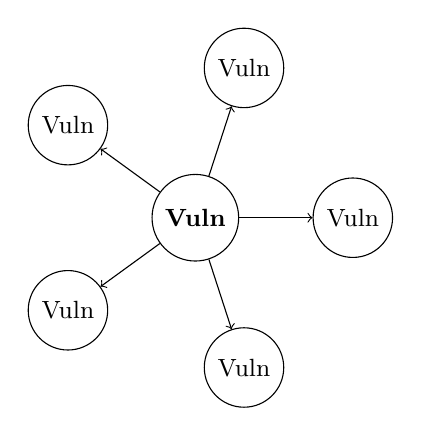
\begin{tikzpicture}

\node[draw, circle] (1) at (360/5 * 0:2cm) {\small Vuln};
\node[draw, circle] (2) at (360/5 * 1:2cm) {\small Vuln};
\node[draw, circle] (3) at (360/5 * 2:2cm) {\small Vuln};
\node[draw, circle] (4) at (360/5 * 3:2cm) {\small Vuln};
\node[draw, circle] (5) at (360/5 * 4:2cm) {\small Vuln};
\node[draw, circle] (6) at (0:0) {\textbf{\small Vuln}};

\path [->] (6) edge node {} (1);
\path [->] (6) edge node {} (2);
\path [->] (6) edge node {} (3);
\path [->] (6) edge node {} (4);
\path [->] (6) edge node {} (5);

\end{tikzpicture}
\end{document}
